\documentclass[11pt]{extarticle}
\usepackage{fullpage} 
\usepackage{microtype}      % microtypography
\usepackage{array}
\usepackage{amsmath,amssymb,amsfonts}
\usepackage{amsthm}
\usepackage{graphicx}
\usepackage[makeroom]{cancel}
\usepackage{mathtools}
\usepackage{caption}

%% Header
\usepackage{fancyhdr}
\fancyhf{}
\fancyhead[C]{CS 136 - 2022s - Final Project Write-up}
\fancyfoot[C]{\thepage} % page number
\renewcommand\headrulewidth{0pt}
\pagestyle{fancy}

\usepackage[headsep=0.5cm,headheight=2cm]{geometry}

%% Hyperlinks always blue, no weird boxes
\usepackage[hyphens]{url}
\usepackage[colorlinks=true,allcolors=black,pdfborder={0 0 0}]{hyperref}

%%% Doc layout
\usepackage{parskip}
\usepackage{times}

%%% Write out problem statements in blue, solutions in black
\usepackage{color}
\newcommand{\officialdirections}[1]{{\color{blue} #1}}

%%% Avoid automatic section numbers (we'll provide our own)
\setcounter{secnumdepth}{0}

%%% Pretty tables
\usepackage{booktabs}

%%% Figure/Table settings
\captionsetup[table]{skip=5pt}
\captionsetup[figure]{labelfont=bf,textfont=it, labelsep=period}
\captionsetup[table]{labelfont=bf}

\begin{document}

\begin{titlepage}
%\begin{vspace}*{\fill}
\begin{center}
{\Large{Tufts University}}
~~\\[7.7 cm]
{\Huge {CS 136 - 2022s}} \\[0.4 cm]
{\Huge {\bf Final Project Write-up}} \\[7.7 cm]
{\Large {\bf Alexander Lobo and Nate Davis}}\\[0.4 cm]
{\Large{May 13, 2022}}
\end{center}
%\end{vspace}*{\fill}
\end{titlepage}

\newpage

\begin{center}
{\Large{\bf Student Names: Alexander Lobo and Nate Davis}}
\end{center}

~~\\

{\Large{\bf Collaboration Statement:}}

Turning in this assignment indicates you have abided by the course Collaboration Policy:

\url{www.cs.tufts.edu/comp/136/2022s/index.html#collaboration-policy}

Total hours spent: 20

We consulted the following resources:
\begin{itemize}
\item Course website
\item Lecture Videos
\item Bishop Textbook
\end{itemize}

\tableofcontents

\newpage
\section{Project Summary}

Our dataset contains 6,598 confirmations (orientations/rotations) of 102 molecules, all of which have been classified in terms of smell as musk or non-musk by human experts. If a molecule has been deemed a musk, all of its confirmations are listed so, and the same is true for non-musks. The dataset is imbalanced, with 5,581 non-musks and 1,016 musks. The features of our dataset comprise 166 measures of intramolecular distance.

We use a logistic regression model with sigmoid link function and multivariate Gaussian prior on the weight vector to predict whether a given confirmation is musk or non-musk. Originally, our learning method was first-order stochastic gradient descent. However, after experiencing some trouble implementing a second-order stochastic gradient descent for our upgrade, we opted to implement batch versions of our methods to compare instead. In order to test for convergence, we calculate a adjusted log loss (which includes a term for the prior) per training example before each weight update and compare it to the log loss from the prior step. If the difference in the log loss between steps becomes less than the predefined threshold or if the maximum iterations is met, then the algorithm terminates.

Our upgrade is a change of learning method to second-order gradient descent. The main problem we seek to address with this upgrade is the time it takes to train our model. Incorporating information from the second derivative of the loss function, as occurs in second-order gradient descent, should allow the model to converge more quickly.

We have made some changes to our first-order gradient descent implementation since checkpoint 2, so we produce new baseline measurements below, but the metrics by which we compare our model pre- and post-upgrade are number of iterations until convergence, time until convergence, and accuracy.

\newpage

\section{Upgrade Implementation}

\subsection{Background}

In Bayesian logistic regression, the Posterior distribution is a useful probability distribution that may be used to predict the probability of certain weight vectors given then occurrence of specific data. It is a powerful tool that allows us to utilize information from the Likelihood (probability of data given weight vector), the Prior (a priori knowledge about the weight vector), the Evidence (marginal probability of the data). One goal of Bayesian reasoning for logistic regression is to find the most probable weight vector that maximizes the probability density of the Posterior, which is known as the MAP estimate. By taking the negative of the Posterior, we can convert our optimization problem from a maximization to a minimization problem by convention. However, unlike with linear regression, the MAP estimate of logistic regression is not known to have an analytical solution. Therefore we depend on optimization methods like gradient descent to solve

\begin{equation}
\hat{\textbf{w}}_{\mathrm{MAP}} = \arg\min_{\textbf{w} \in \mathbb{R}^M} -\ln p(\textbf{w}|\textbf{t}) 
\end{equation}

where $M$ is the feature dimension and $-\ln p(\textbf{w}|\textbf{t})$ is the negative of the posterior distribution.

We then have two options to choose from: first-order and second-order gradient descent. First order gradient descent uses a first-order derivative of the Posterior to make a step change in the weight vector, while second-order gradient descent uses a second-order derivative. Changing the gradient descent method from first-order to second-order is the chosen upgrade to improve the prediction of molecule confirmations as either musk (positive output class) or non-musk (zero output class) smelling.

\subsection{Implementation}

In Checkpoint 3, we derived the following update equations that would be use for our pre- and post-upgrade models using stochastic gradient descent. Each method has two upgrade equations because we originally decided to keep the weight vector and bias term stored as separate variables.

\subsubsection{\textit{First-Order Stochastic Gradient Descent}}

\begin{equation}
\mathbf{w}^{t+1} \leftarrow \mathbf{w}^{t} - \eta \underbrace{\left[ \left(\sigma(\mathbf{w}^t \cdot x_{(i)}) - y_{(i)}\right) x_{(i)} + \alpha \mathbf{w}^{t} \right]}_{g_{(i)}(\mathbf{w}^t)}
\end{equation}

\begin{equation}
c^{t+1} \leftarrow c^{t} - \eta (\sigma(\mathbf{w}^t \cdot x_{(i)}) - y_{(i)})
\end{equation}

\subsubsection{\textit{Second-Order Stochastic Gradient Descent}}

\begin{equation}
\mathbf{w}^{t+1} \leftarrow \mathbf{w}^{t} - \eta \underbrace{\left[r_{(i)}(\mathbf{w^t}) (x_{(i)} \otimes x_{(i)}) + \alpha \right]^{-1}}_{H_{(i)}(\mathbf{w}^t)^{-1}} \underbrace{\left[ \left(\sigma(\mathbf{w}^t \cdot x_{(i)}) - y_{(i)}\right) x_{(i)} + \alpha \mathbf{w}^{t} \right]}_{g_{(i)}(\mathbf{w}^t)}
\end{equation}

\begin{equation}
c^{t+1} \leftarrow c^{t} - \eta \left[ r_{(i)}(\mathbf{w^t}) (x_{(i)} \otimes x_{(i)}) \right]^{-1} \left[ \left(\sigma(\mathbf{w}^t \cdot x_{(i)}) - y_{(i)}\right) \right]
\end{equation}

We found that the first-order stochastic gradient descent update worked quite well, and we were able to show a noisy decrease in the loss function moving towards the global minimum. It seemed promising that a similar result would be achieved for the second-order stochastic gradient descent. Instead, the log loss would always shoot to infinity after a couple iterations regardless of how we tuned the hyperparameters. Our code would specifically error when trying to compute the inverse of the Hessian, throwing a "singular matrix error". We tried debugging the code for a while before concluding that the inverse Hessian calculation does not perform properly when using a single example. Hence, we abandoned the stochastic approach and decided to implement batch gradient descent methods instead. In order to simplify our weight update equations, we also decided to combine the weights and bias terms into a single weight vector so that only a single weight update equation is needed for each method.

To derive the necessary equations for first- and second-order gradient descent, we must revisit the log loss for Bayesian logistic regression that was derived in Checkpoint 3:

\begin{align}
    \ln \mathcal{L}(\mathbf{w}) &= - \left( \sum_{n=1}^N t_n\ln (\sigma(\textbf{w}^\top x_n)) + (1-t_n) \ln (1-\sigma(\textbf{w}^\top x_n)) \right) + \frac{1}{2} \alpha \mathbf{w}^\top \mathbf{w} \\
    &= - \left( \mathbf{t}^\top \ln (\sigma(\mathbf{x} \mathbf{w})) + (1-\mathbf{t})^\top \ln (1-\sigma(\mathbf{x} \mathbf{w})) \right) + \frac{1}{2} \alpha \mathbf{w}^\top \mathbf{w}
\end{align}

\subsubsection{\textit{First-Order Batch Gradient Descent}}

Now, with using Bishop equation (4.91), we can take the gradient of the log loss with respect to $\mathbf{w}$ to obtain

\begin{equation}
     \nabla_\mathbf{w} \ln \mathcal{L}(\mathbf{w}) =  \sum_{n=1}^N \sigma(\textbf{w}^\top x_n) - t_n)x_n + \alpha \mathbf{w}
\end{equation}

Using matrix notation, the gradient of the log loss can be written as

\begin{equation}
     g(\mathbf{w}) = \nabla_\mathbf{w} \ln \mathcal{L}(\mathbf{w}) =  \mathbf{x}^\top (\sigma(\mathbf{x} \textbf{w}) - \mathbf{t}) + \alpha \mathbf{w}
\end{equation}

We can now use the gradient to make a step change given some step-size $\eta$ and iterate until we converge to a solution:

\begin{equation}
\mathbf{w}^{t+1} \leftarrow \mathbf{w}^{t} - \eta \underbrace{\left[ \mathbf{x}^\top (\sigma(\mathbf{x} \textbf{w}^t) - \mathbf{t}) + \alpha \mathbf{w}^t \right]}_{g(\mathbf{w}^t)}
\end{equation}

\subsubsection{\textit{Second-Order Batch Gradient Descent}}

In order to perform second-order gradient descent, we can consider the second-order gradient Hessian matrix $H(\mathbf{w}) \in \mathbb{R}^{M \times M}$ to be

\begin{equation}
H(\mathbf{w}) = \nabla_\mathbf{w} \nabla_\mathbf{w} \ln \mathcal{L}(\mathbf{w})  = \mathbf{x}^\top R(\mathbf{w}) \mathbf{x} + \alpha I_M
\end{equation}

where $R(\mathbf{w}) \in \mathbb{R}^{N \times N}$ is defined as

\begin{equation}
R(\mathbf{w}) =
  \begin{bmatrix}
    \sigma(\textbf{w}^\top x_1)(1-\sigma(\textbf{w}^\top x_1) & & \\
    & \ddots & \\
    & & \sigma(\textbf{w}^\top x_n)(1-\sigma(\textbf{w}^\top x_n)
  \end{bmatrix}
\end{equation}

a diagonal matrix with all 0 off-diagonal entries. Now each update in the weight vector is

\begin{equation}
\mathbf{w}^{t+1} \leftarrow \mathbf{w}^{t} - \eta H(\mathbf{w}^{t})^{-1} g(\mathbf{w}^{t})
\end{equation}

By substituting the formulas given by equation (9) and (11) into the weight update equation, we obtain

\begin{equation}
\mathbf{w}^{t+1} \leftarrow \mathbf{w}^{t} - \eta \underbrace{\left[ \mathbf{x}^\top R(\mathbf{w}) \mathbf{x} + \alpha I_M \right]^{-1}}_{H(\mathbf{w}^t)^{-1}} \underbrace{\left[ \mathbf{x}^\top (\sigma(\mathbf{x} \textbf{w}) - \mathbf{t}) + \alpha \mathbf{w} \right]}_{g(\mathbf{w}^t)}
\end{equation}

\subsubsection{\textit{Code Implementation}}

Now, the following steps are taking to implement the first- and second-order batch gradient descent learning algorithm:

\begin{enumerate}
\item Initialize the python class \texttt{MAPEstimator()} with parameters (e.g. prior weight vector, solver type, maximum iterations, convergence tolerance, step size, etc.)
\item Use \texttt{if} statement to determine if the solver type is first-order (\texttt{'fo'}) or second-order (\texttt{'so'}).
\item initialize loop counting parameter to keep track of number of iterations and initialize loss array to keep track of log loss changes between iteration steps.
\item Transform the training dataset to include a column of ones (this gets matrix multiplied by the bias term in the weight vector).
\item Initiate \texttt{while} loop.
\item Use equation (10) or equation (14) to perform the weight update, depending on the solver method.
\item Compute updated log loss using updated weight vector.
\item Iterate until maximum iterations are reached or the difference in log loss between steps becomes less than the pre-defined tolerance.
\end{enumerate}

\subsection{Bottlenecks}

\subsubsection{\textit{Stochastic vs. Batch Gradient Descent}}

As discussed before, one of the issues we ran into was getting our second-order stochastic gradient descent method to converge. Although we could not figure out the issue (or even determine if it is even feasible), we addressed this issue by pivoting our project to focus on batch first and second-order gradient descent. Although we had to spend a bit of extra time to re-implement our pre-upgrade code, we are now able to obtain and analyze the results for both methods.

\subsubsection{\textit{Training Time}}

Considering that the computational complexity ($O(m^3)$) of second-order gradient descent, we expected the second-order method to take a bit longer to converge than the first-order method when the hyperparameters are not optimally set. However, we instead found that the second-order method took much longer than expected. The second-order method is also a lot more sensitive to the step-size than the first order method is. As a result, it was much more difficult to tune the hyperparameters for the second-order method. Considering how long each grid search would take (10 minutes on average), we ultimately decided to limit the maximum iterations to 100 to save time.

\newpage

\section{Performance Hypotheses for Upgrade}

\textbf{Hypothesis 1:} We hypothesize that our upgrade from first- to second-order gradient descent will cause our model to converge in fewer iterations because second-order gradient descent's incorporation of the second-degree derivative of the loss function should make each step more efficient in minimizing the loss.

\begin{itemize}
\item Our implementation of gradient descent keeps track of the number of iterations until convergence, and we look at the distribution of these counts over k-fold cross validation with 10 folds.
\end{itemize}

\textbf{Hypothesis 2:} We hypothesize that our upgrade to second-order gradient descent will cause our model to converge in less time because, although time complexity of one step of second-order gradient descent is $O(m^3)$, versus $O(m)$ for first-order gradient descent (with $m$ being the size of the weight vector), the aforementioned incorporation of second-degree derivative information should lower the total number of steps 

\begin{itemize}
\item We calculate runtime until convergence using the python \texttt{time()} function for each of the 10 iterations in our k-fold cross validation.
\end{itemize}

\textbf{Hypothesis 3:} We hypothesize that our upgrade to second-order gradient descent will have no major effect on the accuracy of our model, as in theory it should converge to the same minimum as first-order gradient descent, just faster.

\begin{itemize}
\item We measure accuracy on held-out data via k-fold cross validation with 10 folds.
\end{itemize}

~~\\


\newpage

\section{Evaluating hypotheses for upgrade}

For each of our hypotheses, we used the following hyperparameters for our learning methods:

\begin{center}
\begin{table}[h]
\centering
\caption{Optimized Hyperparameters}
\begin{tabular}{lrr}
\hline
                & \multicolumn{2}{l}{Gradient Descent Method}                          \\ 
\hline
\hline
Hyperparameter  & \multicolumn{1}{l}{First-Order~} & \multicolumn{1}{l}{Second-Order}  \\ 
\hline
step size ($\eta$) & 0.0001                           & 0.1                               \\
$\alpha$           & 1                                & 1                                 \\
max. iterations    & 1000                             & 100                              \\
tolerance          & 0.00001                          & 0.01                              \\
\hline
\end{tabular}
\end{table}
\end{center}

Our goal with the hyperparameters we chose was to get as close to an apples to apples comparison as possible between first-order and second-order gradient descent. To start, we used grid search to optimize step size, $\alpha$, and tolerance for the accuracy of first-order gradient descent. We also set the maximum number of iterations high enough such that none of our runs hit it. 

Our thought was that, using these same values, we could fairly test second-order gradient descent in comparison. We found, however, that with the same tolerance and step size, second-order gradient descent took an incredibly long amount of time, but that it could achieve similar or better heldout accuracy in fewer iterations when we raised these values. Therefore, we raised step size to 0.1 and tolerance to 0.01. Our thought as to why this might be required is that the inclusion of the inverse Hessian in the weight update formula for second order gradient descent might bring effective step size down a few orders of magnitude. Regardless, tweaking these values didn't change the results of our hypothesis tests, directionally speaking.

\newpage

\subsection{Hypothesis 1}

We hypothesized that using second-order gradient descent, our model would converge in fewer iterations. To evaluate this hypothesis, we performed k-fold cross validation with 10 randomly selected folds on our model using both first- and second- order gradient descent. For each of the 10 folds, we tracked the number of iterations it took to converge.

\begin{figure}[h!]
\begin{center}
    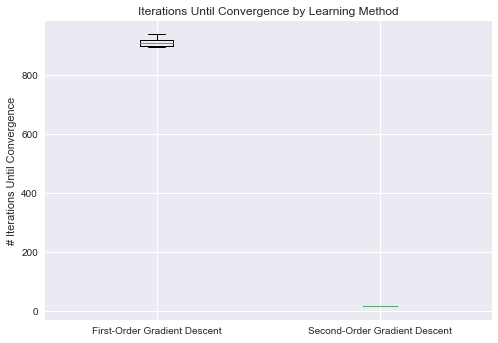
\includegraphics[scale=.7]{iterations.png}
    \caption{Held-out accuracy rate by learning method}
     \label{fig:x}
\end{center}
\end{figure}

Every run of first-order gradient took almost two orders of magnitude more iterations than second-order gradient descent to converge, with each first-order run taking about 900 iterations and each second-order run taking ~20.

This result was in line with our hypothesis, though we did not expect the difference in magnitude to be this great. True to theory, incorporating second derivative information on the loss function certainly appears to have made each weight update more efficient. Even when we used the same step size and tolerance values for second-order gradient descent, this result held. 

\newpage

\subsection{Hypothesis 2}

We hypothesized that using second-order gradient descent, our model would converge in less time. To evaluate this hypothesis, we performed k-fold cross validation with 10 randomly selected folds on our model using both first- and second- order gradient descent. For each of the 10 folds, we tracked the time it took for the model to converge using the time() function in Python.

\begin{figure}[h!]
\begin{center}
    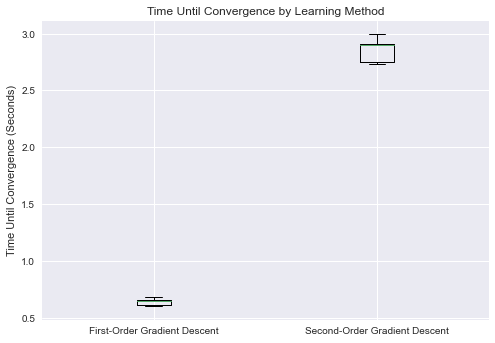
\includegraphics[scale=.7]{time.png}
	\caption{Time until convergence by learning method}    
    \label{fig:x}
\end{center}
\end{figure}

In contrast to number of iterations, every run of second-order gradient descent took approximately 4 times longer than each run of first-order gradient descent.

This result, paired with the results of hypothesis test 1, shows that, although first-order gradient descent took approximately 45 times as many iterations to converge, it still took about 4 times longer for runs of second-order gradient descent to converge. These two findings imply that each iteration of second-order gradient descent took roughly 180 times longer than a single iteration of first-order gradient descent. That the weight vector had $m = 167$ dimensions, and a single iteration of second-order gradient descent is supposed to take $O(m^3)$ versus $O(m)$ for a single iteration of first-order gradient descent, we would in fact expect a single iteration to take $167^2 \approx$ 28,000 times longer. So, in theory, our second-order learning method ought to have taken even \textit{longer} relative to first-order (and it certainly would have if we had kept step size and tolerance constant, though not to this extent).

Our hypothesis certainly proved false, though at this point we are not exactly sure why. There is obviously something about the nature of second-order (and/or first-order) gradient descent, or about our implementation of it, that we do not fully understand, or else these results would be easier to reconcile.

\newpage

\subsection{Hypothesis 3}

We hypothesized that using second-order gradient descent, our model would exhibit similar accuracy. To evaluate this hypothesis, we performed k-fold cross validation with 10 randomly selected folds on our model using both first- and second- order gradient descent. For each of the 10 folds, we tracked score the accuracy of our model on the held-out data.

\begin{figure}[h!]
\begin{center}
    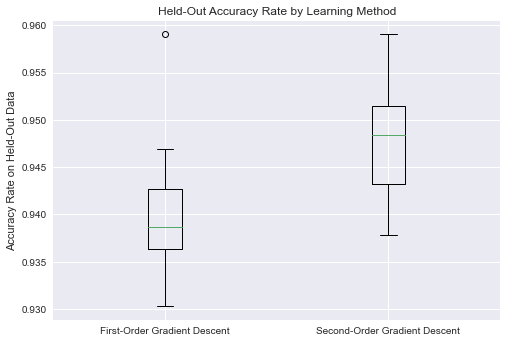
\includegraphics[scale=.7]{accuracy.png}
    \caption{Held-out accuracy rate by learning method}
    \label{fig:x}
\end{center}
\end{figure}

While each method exhibited a range of accuracy, second-order gradient descent on average converged to a higher accuracy rate.

This result implies that second-order gradient descent is able to get closer to the global minimum of the loss gradient, even with higher step size and tolerance levels. Perhaps this confirms that the inverse Hessian term in the weight update formula for second-order gradient descent acts as a sort of dynamic step size factor as we approach the global minimum, enabling it to delve deeper and more precisely into the minimum. This is strange as our tolerance for second-order gradient descent was three orders of magnitude higher than that for first-order. Perhaps on the last weight update for second-order, however, the method gets incredibly close to the actual global minimum, relative to first-order, and the last change in loss is still much smaller for second-order.

We failed to confirm our hypothesis here, although we were somewhat imprecise about wording it. The accuracy on heldout data for each learning method is certainly in the same neighborhood--all values fall between 0.93 and 0.96. That said, the accuracy associated with second-order gradient descent certainly appears to be generally higher. If we were to redo this hypothesis, we might be well served by defining more carefully what constitutes same or similar accuracy.

\newpage

\section{Reflection}

TODO: Complete Reflection

In this section, you should reflect on your project in 2-3 paragraphs, being sure to answer the following questions:
\begin{itemize}
	\item Did anything about how your original model worked on your data surprise you? (3 points)
	\item What about your upgrade? (3 points)
	\item If you were to continue working with this data, what would you like to try next?  Why? (3 points)
\end{itemize}

This section should 1/2-2/3 of a page long.

\end{document}

